\section{单边雅可比算法实现 SVD}

上一章给出了奇异值分解（Singular Value Decomposition, SVD）的存在性结论：
任意矩阵 $A\in\mathbb{R}^{m\times n}$ 都可以写成 $A=U\Sigma V^T$。
然而，存在性本身并不构成可执行算法。数值线性代数更关心的是：
在浮点数运算（floating-point arithmetic）中，如何以可控的舍入误差、可接受的计算复杂度，
以及与目标硬件相匹配的访存模式，稳定地构造这一分解。

本章首先从算法谱系的角度定位主流 SVD 方法，随后说明本项目选择单边雅可比
（one-sided Jacobi）路线的原因。之后，我们给出该方法的数学模型、几何解释与串行伪代码；
后续章节将在此基础上讨论其 CUDA 并行化。

\subsection{SVD 算法谱系}

SVD 算法大体可以按“先规约再求解”与“直接正交化”两类思路理解。不同方法之间并不存在
单一维度上的绝对优劣；它们分别在精度、吞吐、并行性、实现复杂度以及目标矩阵规模之间采取不同折中。

\paragraph{双对角化加 QR 迭代。}
经典密集矩阵 SVD 通常先用 Householder 反射（Householder reflection）把 $A$ 规约为双对角矩阵
（bidiagonal matrix）：
\[
    A = QBP^T,
\]
其中 $Q$、$P$ 为正交矩阵，$B$ 仅在主对角线与一条副对角线上非零。随后，对 $B$ 执行隐式 QR 迭代
（implicit QR iteration）或相关变体。该路线理论成熟、数值稳定，是 LAPACK 等基础线性代数库的重要实现路径。
其主要局限在于：规约阶段与迭代阶段包含较强的数据依赖，直接映射到 GPU 时难以充分暴露细粒度并行性。

\paragraph{分治法。}
分治 SVD（divide-and-conquer SVD）同样从双对角矩阵出发，将问题拆分为较小子问题，
再通过秩一修正（rank-one modification）合并结果。对于需要全部奇异向量的中大型密集矩阵，
该方法通常具有较高效率。相应代价是实现复杂度与工作空间需求较高，且合并阶段包含较精细的数值处理。

\paragraph{MRRR 与相关特征值路线。}
部分实现会把 SVD 转化为对称特征值问题（symmetric eigenvalue problem），例如处理
$A^TA$ 或增广矩阵
\[
    \begin{bmatrix}
        0   & A \\
        A^T & 0
    \end{bmatrix}.
\]
MRRR（Multiple Relatively Robust Representations）等方法在特征值问题中具有重要地位。
不过，显式形成 $A^TA$ 会导致条件数平方化：
\[
    \kappa_2(A^TA)=\kappa_2(A)^2,
\]
从而使小奇异值对应的方向更容易被舍入误差淹没。对于强调奇异向量鲁棒性的实现，这通常不是理想选择。

\paragraph{Krylov 与随机化方法。}
当矩阵规模极大且只需要前 $k$ 个奇异值或低秩近似时，Lanczos 双对角化（Lanczos bidiagonalization）、
块 Krylov 方法（block Krylov method）与随机 SVD（randomized SVD）具有较强吸引力。
它们并不追求完整分解，而是通过矩阵-向量乘法或矩阵-块乘法提取主子空间。
这类方法适用于稀疏矩阵、大规模机器学习与近似压缩；但本项目的目标是实现一个结构清晰、
结果完整且便于验证的 dense SVD kernel，因此它们不是本文的算法主线。

\paragraph{雅可比方法。}
雅可比方法（Jacobi method）通过一系列二维正交旋转逐步消除非对角相关项。面向 SVD 时，
常见形式包括双边雅可比（two-sided Jacobi）与单边雅可比：前者对对称矩阵或增广结构做左右旋转，
后者直接旋转 $A$ 的列，使列向量逐步正交。雅可比方法通常不是浮点操作次数最少的选择，
但它具有两个对本项目尤其关键的性质：良好的正交性保持能力，以及高度局部的计算结构。
对于 GPU，这种局部性意味着互不共享列的列对可以被组织为并行任务。

\subsection{为什么选择单边雅可比}

本项目选择单边雅可比，并不是因为它在所有问题规模上都具有最高吞吐，而是因为它与本项目的设计目标高度一致：
避免不必要的条件数放大，直接控制列正交性，并提供可验证、可并行化的局部计算原语。

\paragraph{第一，避免显式形成 $A^TA$。}
上一章的存在性证明借助 $A^TA$，但算法实现并不需要显式构造它。单边雅可比在每个列对
$(p,q)$ 上只计算三个标量：
\[
    \alpha=a_p^Ta_p,\qquad
    \beta =a_q^Ta_q,\qquad
    \gamma=a_p^Ta_q.
\]
这等价于读取 $2\times 2$ 的局部 Gram 矩阵（Gram matrix）信息，而不是构造完整的 $A^TA$。
因此，该方法避免了条件数平方化所带来的系统性数值风险。

\paragraph{第二，正交性是算法的主目标，而不是副产品。}
SVD 的核心不仅是获得奇异值，还包括构造高质量的左右奇异子空间。单边雅可比的每一步都直接降低列向量之间的相关性；
收敛时，当前矩阵的列已近似两两正交。于是左奇异向量可由列归一化得到：
\[
    \sigma_j=\|a_j\|_2,\qquad u_j=a_j/\sigma_j.
\]
该路线的状态含义十分明确：右奇异矩阵 $V$ 由旋转累积而来，奇异值来自列范数，左奇异矩阵来自归一化后的工作矩阵列。

\paragraph{第三，旋转是局部原语。}
一次 Jacobi 旋转只修改两列 $a_p,a_q$，以及右奇异矩阵中的两列 $v_p,v_q$。
如果一轮中选出的列对互不重叠，例如
\[
    (1,2),(3,4),(5,6),\ldots,
\]
则这些旋转之间不存在写冲突，可以并行执行。这个性质自然导向后续章节讨论的巡回赛排序
（tournament ordering / round-robin ordering）：它把所有列对分批组织成无冲突的 matching。

\paragraph{第四，代码路径容易验证。}
从工程角度看，单边雅可比的优势还在于状态空间有限且可观测。算法只需要维护当前工作矩阵
$A^{(k)}$、累积右旋转 $V^{(k)}$、容差 $\varepsilon$ 与扫描轮次（sweep count）。
每次旋转之后，可以检查局部 Gram 矩阵的非对角项是否下降；每个 sweep 之后，可以检查整体列正交残差。
这使得教学推导、单元测试以及 CUDA kernel 调试都具有清晰的验证接口。

\subsection{数学模型}

设初始矩阵为
\[
    A^{(0)}=A,\qquad V^{(0)}=I_n.
\]
单边雅可比维护如下不变量：
\[
    A^{(k)} = A V^{(k)},
\]
其中 $V^{(k)}$ 是若干个平面旋转（plane rotation）的乘积，因此始终保持正交。
当 $A^{(k)}$ 的列两两正交时，有
\[
    \bigl(A^{(k)}\bigr)^T A^{(k)}
    =
    \bigl(V^{(k)}\bigr)^T A^T A V^{(k)}
    =
    \operatorname{diag}(\sigma_1^2,\ldots,\sigma_n^2),
\]
于是 $V^{(k)}$ 的列给出右奇异向量，$A^{(k)}$ 的列范数给出奇异值。

现在考虑一对列 $(p,q)$。记
\[
    a=a_p,\qquad b=a_q,
\]
并定义局部 Gram 矩阵
\[
    H =
    \begin{bmatrix}
        \alpha & \gamma \\
        \gamma & \beta
    \end{bmatrix}
    =
    \begin{bmatrix}
        a^Ta & a^Tb \\
        a^Tb & b^Tb
    \end{bmatrix}.
\]
目标是构造一个二维正交旋转
\[
    G =
    \begin{bmatrix}
        c  & s \\
        -s & c
    \end{bmatrix},
    \qquad c^2+s^2=1,
\]
使更新后的两列
\[
    [a'_p,a'_q]=[a_p,a_q]G
\]
满足
\[
    (a'_p)^T a'_q = 0.
\]
等价地，要求
\[
    G^T H G
\]
的非对角元为 $0$。

令 $t=s/c$。直接展开可得非对角元为
\[
    \gamma(c^2-s^2)+(\alpha-\beta)cs.
\]
若 $\gamma\ne0$，令该项为 $0$，得到
\[
    \gamma t^2 +(\beta-\alpha)t-\gamma=0.
\]
设
\[
    \tau=\frac{\beta-\alpha}{2\gamma},
\]
则
\[
    t^2+2\tau t-1=0.
\]
为避免在 $|\tau|$ 很大时发生灾难性抵消（catastrophic cancellation），采用稳定形式
\[
    t =
    \begin{cases}
        \dfrac{1}{\tau+\sqrt{1+\tau^2}},   & \tau\ge0, \\[1.2em]
        -\dfrac{1}{-\tau+\sqrt{1+\tau^2}}, & \tau<0,
    \end{cases}
\]
然后计算
\[
    c=\frac{1}{\sqrt{1+t^2}},\qquad s=tc.
\]
若 $\gamma$ 已经足够小，则跳过旋转。实际实现中常采用相对准则
\[
    |\gamma|\le \varepsilon\sqrt{\alpha\beta},
\]
其中 $\varepsilon$ 为容差。相比绝对阈值，该准则会随列范数自动缩放，因此在不同矩阵尺度下更加稳健。

一次旋转的列更新为
\[
    a'_p = c a_p - s a_q,\qquad
    a'_q = s a_p + c a_q,
\]
右奇异向量矩阵同步更新为
\[
    v'_p = c v_p - s v_q,\qquad
    v'_q = s v_p + c v_q.
\]
这里的 $V$ 并不是后处理阶段补写的记录表，而是算法不变量的一部分：
每次 $A$ 右乘 $G$，$V$ 也右乘同一个 $G$，从而始终保持 $A^{(k)}=AV^{(k)}$。

\subsection{几何理解}

单边雅可比的几何图像是：在输入空间中持续旋转坐标轴，使这些坐标轴经过 $A$ 映射后，
在输出空间中逐步变为互相正交的向量。

对列对 $(a_p,a_q)$ 而言，当前两个输入基方向 $e_p,e_q$ 经过 $A^{(k)}$ 后成为输出向量
$a_p,a_q$。若 $a_p^Ta_q\ne0$，说明这两个输出方向尚未正交。Jacobi 旋转并不直接在输出空间中修改
这两个向量的几何关系，而是在输入平面 $\operatorname{span}\{e_p,e_q\}$ 内选择一组新的正交坐标：
\[
    e'_p = c e_p - s e_q,\qquad
    e'_q = s e_p + c e_q.
\]
在新坐标下，
\[
    A e'_p = a'_p,\qquad A e'_q = a'_q,
\]
且这两个输出向量被构造为正交。

因此，单边雅可比并不是对奇异向量进行启发式猜测；它是在逐步寻找一组输入正交基，使 $A$ 将该基映射为
一组输出正交向量。当所有列对都满足正交条件后，
\[
    A V = [\sigma_1u_1,\ldots,\sigma_nu_n].
\]
此时每个列向量的方向给出 $u_i$，长度给出 $\sigma_i$。该过程与上一章存在性证明的逻辑一致：
证明中一次性调用谱定理，而算法中则通过一系列局部旋转逐步构造同一结构。

\subsection{伪代码}

下面的伪代码描述串行版本。CUDA 版本不会让线程任意竞争列资源，而是把列对组织为无冲突批次；
但其数学核心仍然是同一个二维正交旋转。

\begin{pseudolisting}
    algorithm OneSidedJacobiSVD(A, epsilon, max_sweeps)
    input:
    A: real m by n matrix
    epsilon: relative orthogonality tolerance
    max_sweeps: upper bound on sweeps
    output:
    U: left singular vectors
    Sigma: singular values
    V: right singular vectors

    begin
    V = Identity(n)
    converged = false
    sweeps = 0

    while not converged and sweeps < max_sweeps do
    converged = true
    sweeps = sweeps + 1

    for p = 0 to n - 2 do
    for q = p + 1 to n - 1 do
    alpha = dot(A[:, p], A[:, p])
    beta  = dot(A[:, q], A[:, q])
    gamma = dot(A[:, p], A[:, q])

    threshold = epsilon * sqrt(alpha * beta)
    if abs(gamma) > threshold then
    converged = false

    tau = (beta - alpha) / (2 * gamma)
    if tau >= 0 then
    t = 1 / (tau + sqrt(1 + tau * tau))
    else
    t = -1 / (-tau + sqrt(1 + tau * tau))
    end if

    c = 1 / sqrt(1 + t * t)
    s = t * c

    for i = 0 to m - 1 do
    old_p = A[i, p]
    old_q = A[i, q]
    A[i, p] = c * old_p - s * old_q
    A[i, q] = s * old_p + c * old_q
    end for

    for i = 0 to n - 1 do
    old_p = V[i, p]
    old_q = V[i, q]
    V[i, p] = c * old_p - s * old_q
    V[i, q] = s * old_p + c * old_q
    end for
    end if
    end for
    end for
    end while

    for j = 0 to n - 1 do
    Sigma[j] = norm2(A[:, j])
    if Sigma[j] > epsilon then
    U[:, j] = A[:, j] / Sigma[j]
    else
    U[:, j] = ZeroVector(m)
    end if
    end for

    return U, Sigma, V
    end
\end{pseudolisting}

该版本刻意保留朴素的双重列对循环，以便直接呈现算法不变量。后续 GPU 章节会把
$(p,q)$ 的遍历方式替换为巡回赛排序，使同一批次中的列对互不重叠，从而将“局部旋转”提升为
“批量并行旋转”。算法本体保持不变；改变的是调度方式与硬件映射。

\begin{figure}[htbp]
    \centering
    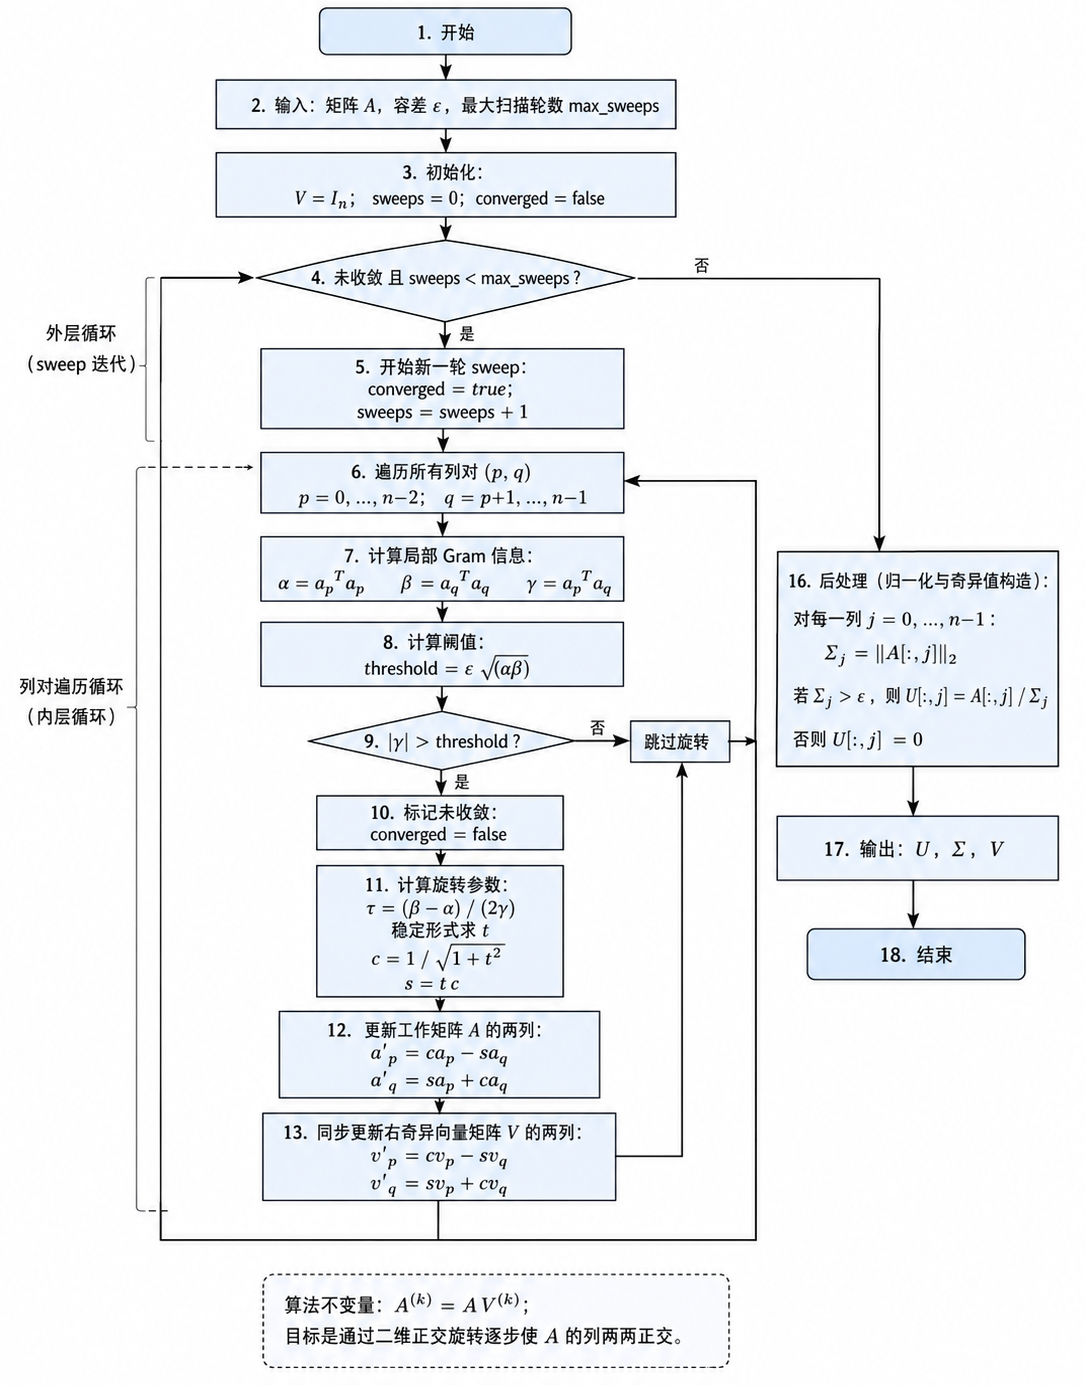
\includegraphics[width=0.92\textwidth]{figures/one-sided-jacobi.png}
\end{figure}

\subsection{复杂度分析}

复杂度分析需要区分两个层次：一是固定一次 sweep 内的代价，二是算法达到给定容差所需的 sweep 数。
前者可以由循环结构直接得到；后者依赖矩阵谱分布、奇异值间隔、初始列相关性以及容差 $\varepsilon$，
通常不能仅由 $m,n$ 给出一个紧致的先验界。因此，工程实现中通常以 \texttt{max\_sweeps} 作为外部上界，
并用列正交残差作为实际停止准则。

对一个固定列对 $(p,q)$，算法首先计算
\[
    \alpha=a_p^Ta_p,\qquad
    \beta=a_q^Ta_q,\qquad
    \gamma=a_p^Ta_q.
\]
这三个量可以在一次行扫描中同时累加，因此统计阶段的代价为 $O(m)$。若该列对已经满足
\[
    |\gamma|\le \varepsilon\sqrt{\alpha\beta},
\]
则本次列对处理到此结束；若需要旋转，则还要更新 $A$ 的两列，代价为 $O(m)$，
并同步更新 $V$ 的两列，代价为 $O(n)$。因此，一个列对的代价可以写成
\[
    O(m) + \mathbf{1}_{\mathrm{rot}}\,O(m+n),
\]
其中 $\mathbf{1}_{\mathrm{rot}}$ 表示该列对是否实际执行旋转。

一次 sweep 会访问所有列对。列对总数为
\[
    N_p=\frac{n(n-1)}{2}=O(n^2).
\]
若第 $s$ 次 sweep 中实际旋转的列对数量为 $r_s$，则该 sweep 的代价为
\[
    O(mn^2)+O\bigl(r_s(m+n)\bigr),
    \qquad 0\le r_s\le N_p.
\]
在最坏情况下，几乎所有列对都需要旋转，于是单次 sweep 的上界为
\[
    O(mn^2+n^3).
\]
这里的 $O(mn^2)$ 来自列点积统计与工作矩阵 $A$ 的列更新，$O(n^3)$ 来自右奇异矩阵 $V$ 的累积更新。
若只需要奇异值而不需要显式右奇异向量，则可以省略维护 $V$，相应的 $O(n^3)$ 项也会消失。
但本项目输出完整 thin SVD，因此必须保留这一项。

设算法在给定容差下执行了 $T$ 次 sweep。忽略初始化常数后，主迭代阶段的总时间复杂度为
\[
    O\bigl(T(mn^2+n^3)\bigr).
\]
收敛后的后处理需要计算每一列的范数并归一化：
\[
    \sigma_j=\|a_j\|_2,\qquad u_j=a_j/\sigma_j,
\]
总成本为 $O(mn)$。因此完整串行算法的总体复杂度可写为
\[
    O\bigl(T(mn^2+n^3)+mn\bigr),
\]
其中 $T\le \texttt{max\_sweeps}$，但其实际值由输入矩阵和容差共同决定。

空间复杂度方面，工作矩阵 $A$ 需要 $O(mn)$ 存储，右奇异矩阵 $V$ 需要 $O(n^2)$，
输出左奇异矩阵 $U$ 需要 $O(mn)$，奇异值数组 $\Sigma$ 需要 $O(n)$。若原地覆盖工作矩阵并把输出计入总空间，
则存储复杂度为
\[
    O(mn+n^2).
\]
对于 thin SVD 的典型场景 $m\ge n$，该空间界与输出规模同阶；也就是说，算法并没有引入超过结果本身数量级的额外长期存储。

这个复杂度结论也解释了为什么下一章要强调调度与规约。单边雅可比的数学原语很局部，
但每个 sweep 覆盖 $O(n^2)$ 个列对；如果仍按串行顺序执行，局部性并不会自动转化为吞吐。
GPU 并行化的核心价值，正是把同一 sweep 中互不冲突的列对组织为批量任务，
在不破坏算法不变量的前提下压缩墙钟时间（wall-clock time）。
